\section{Hyperparameter surfaces}
\label{app:surfaces}

\paragraph{The bootstrap selection protocol, self-contained.}
Following \citet{oliveira2025}: (1) take each configuration's
in-sample \emph{quarterly} return series; (2) moving-block bootstrap
--- blocks of four consecutive quarters, preserving short-range
autocorrelation and volatility clustering, $B=2{,}000$ resamples;
(3) \emph{coupled} indices: the same resample paths for every
configuration, so cross-config differences are configuration
effects, not resampling luck; (4) compute the utility (Sharpe, or IR
for the long-only product) on each resample, giving one distribution
per configuration; (5) select on the 5th percentile --- a
configuration wins only by being good in its bad resamples, which
penalizes performance concentrated in a few lucky quarters
(the winner's-curse correction that a point-estimate maximum lacks).
The choice is then frozen and evaluated on untouched years. Scope
and limits, stated plainly: the bootstrap is a robust \emph{ranking}
criterion, never a source of formal inference (all $p$-values in
this report are Newey--West); block length (one year) and the
percentile were fixed a priori; at $T\approx30$ the percentile
tracks the point estimate (reported as an honest null); and the
protocol assumes a stationary utility distribution --- an assumption
it can itself audit through the cross-configuration in-sample to
held-out rank correlation, which validated selection once (NCB,
$+0.53$) and refused it twice (FSS, LO tilt).

\begin{figure}[h]
\centering
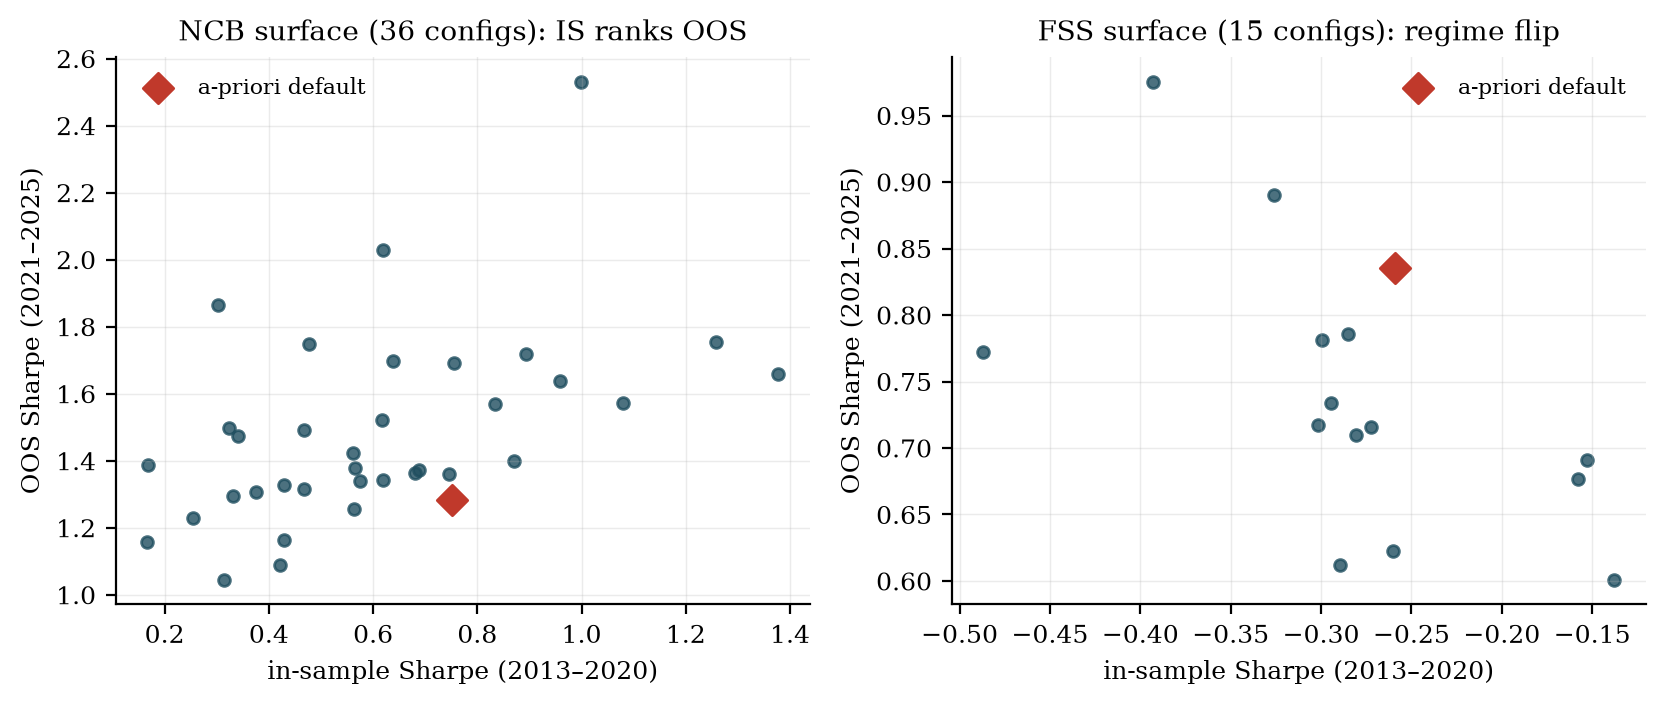
\includegraphics[width=.95\linewidth]{figs/f7_surfaces.png}
\caption{In-sample (2013--2020) versus out-of-sample (2021--2025)
Sharpe by configuration. Left: NCB, 36 configurations --- the whole
surface is OOS-positive and the in-sample ordering predicts the OOS
ordering (rank corr.\ $+0.53$); selection is meaningful, the default
(diamond) is conservative mid-surface. Right: FSS, 15 configurations
--- the surface moves as one block across a regime flip and the IS
ordering \emph{anti-predicts} OOS (rank corr.\ $-0.81$): the correct
use of the selection protocol is to refuse to select.}
\label{fig:surfaces}
\end{figure}

\begin{table}[h]
\centering\scriptsize
\caption{NCB surface, top rows and default (full 36-row table in the
repository). Coupled moving-block bootstrap (block 4, $B=2{,}000$);
selection statistic $=$ 5th percentile of bootstrap Sharpe.}
\begin{tabular}{lrrrrr}
\toprule
config (w-quantile / growth / min holders) & IS Sharpe & boot p05 &
OOS Sharpe & OOS $t$ \\
\midrule
0.95 / 1.50 / 3 (both selectors' pick) & $+1.38$ & $+0.92$ & $+1.66$ & $+4.85$ \\
0.95 / 1.50 / 5 & $+1.26$ & $+0.72$ & $+1.76$ & $+5.08$ \\
0.95 / 1.50 / 10 (best OOS) & $+1.00$ & $+0.49$ & $+2.53$ & $+5.44$ \\
\textbf{0.90 / 1.25 / 5 (a-priori default)} & $+0.75$ & $+0.14$ & $+1.28$ & $+3.31$ \\
worst on grid & $+0.17$ & $-0.34$ & $+1.39$ & $+3.93$ \\
\bottomrule
\end{tabular}
\end{table}

\begin{table}[h]
\centering\scriptsize
\caption{FSS surface (threshold $\times$ basket fraction),
index-hedged short-leg Sharpe. All fifteen configurations lose
modestly in-sample and pay out-of-sample: a regime, not a
hyperparameter.}
\begin{tabular}{lrrrr}
\toprule
config & IS Sharpe & boot p05 & OOS Sharpe & OOS $t$ \\
\midrule
$-$0.05 / top 10\% & $-0.14$ & $-0.57$ & $+0.60$ & $+1.87$ \\
\textbf{$-$0.10 / top 20\% (default)} & $-0.26$ & $-0.75$ & $+0.84$ & $+2.84$ \\
$-$0.20 / top 20\% (best OOS) & $-0.39$ & $-1.05$ & $+0.98$ & $+4.02$ \\
\bottomrule
\end{tabular}
\end{table}
